\section{Analyse}

\subsection{Korrektheitsbeweis}

\subsubsection{Betrachtung des Algorithmus} \label{algo_analyse}

In Abb. \ref{definition_kausal} ist der Algorithmus für einen kausalen Multicast beschrieben.

\begin{figure}[htbp]
\begin{center}
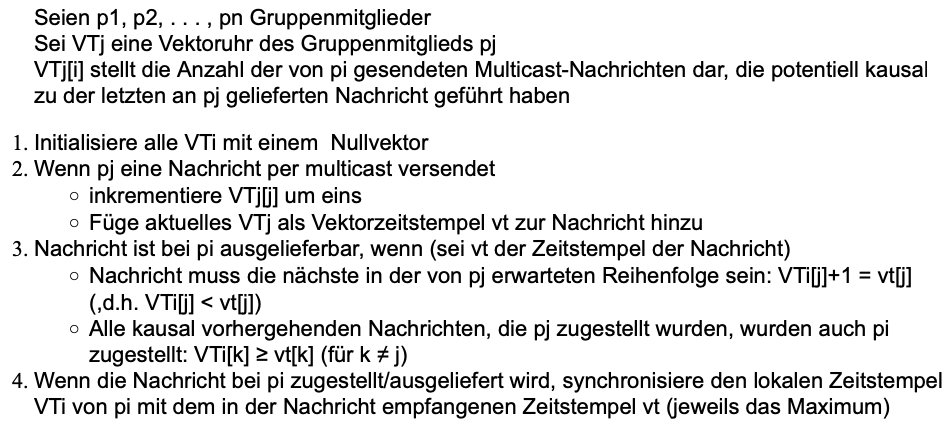
\includegraphics[scale=0.4]{Latex/Bilder/Definition.png}
\caption{\label{definition_kausal} Algorithmus für einen kausalen Multicast \cite{Aufgabenstellung}}
\end{center}
\end{figure}

Aus diesem gehen die folgenden wesentlichen Merkmale hervor:

\begin{itemize}
    \item Alle Prozesse werden mit einem sogenannten Nullvektor initialisiert,
    \item Inkrementiere die eigene Vektoruhr $VTj[j]$ um 1 beim Versenden einer Nachricht,
    \item Eine Nachricht ist in einem Prozess $pi$ auslieferbar, wenn
        \begin{enumerate}
            \item dessen Vektoruhr an der Position j (j = Identität von $pj$) um 1 höher ist als der Zeitstempel der Nachricht: $VTi[j]+1 = vt[j]$,
            \item alle Nachrichten, die kausal vor der aktuellen Nachricht stehen, bereits bei $pi$ angekommen und verarbeitet worden sind. Sichergestellt wird dies durch die Bedingung $VTi[k]\geq vt[k]$ für $k \neq j$.
        \end{enumerate}
    \item Synchronisiere den lokalen Zeitstempel des Prozesses beim Ausliefern einer Nachricht mit dem der ausgelieferten Nachricht.
\end{itemize}

\paragraph{Initialisierung mit Nullvektor}

Die Eindeutigkeit jedes Prozesses wird über die Vektoruhr Zentrale kontrolliert. Durch das Mapping der Prozess ID auf die Vektoruhr ID hat jeder Prozess eine eindeutige Vektoruhr ID. Die Nullvektoren haben entsprechend alle eine unterschiedliche Länge und sind ausschließlich mit Nullen gefüllt.

\paragraph{Inkrementierung beim Versenden}

Die Inkrementierung der Vektoruhr ist im \textit{Prozess der Queues} implementiert. Die entsprechende Schnittstelle wird ausschließlich in der \textit{receive}-Schnittstelle der \textit{send} Funktion (siehe Kapitel \ref{cbcast_send_realisierung}) aufgerufen. Das Versenden eine Nachricht ist nur über diese Funktion möglich.

\paragraph{Auslieferung der Nachrichten}

\begin{figure}[htbp]
\begin{center}
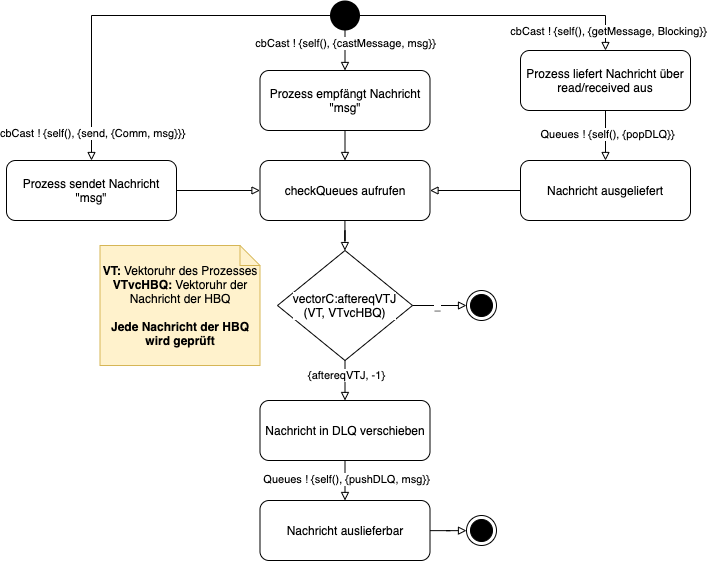
\includegraphics[scale=0.55]{Latex/Bilder/Auslieferbarkeit.png}
\caption{\label{auslieferbarkeit_analyse} Auslieferbarkeit}
\end{center}
\end{figure}

In Abb. \ref{auslieferbarkeit_analyse} ist dargestellt, wann genau Nachrichten ausgeliefert werden können und wann Nachrichten ausgeliefert werden.\\
Auslieferbar sind ausschließlich Nachrichten, welche in der \textit{Delivery Queue} gespeichert sind. Geprüft ob Nachrichten in die \textit{Delivery Queue} verschoben werden dürfen, wird, bei jeder Veränderung der \textit{Holdback} oder \textit{Delivery Queue} über die Funktion \textit{checkQueues}. Verschoben werden ausschließlich Nachrichten dessen Vektoruhr an der Position j (j = Identität des Prozesses) um 1 kleiner sind als der Zeitstempel des Prozesses: $VTi[j]+1 = vt[j]$. Dies wird durch die Funktion \textit{vectorC:aftereqVTJ/2} sichergestellt.\\
Die Kausalität bleibt durch die Implementierung der \textit{Delivery Queue} als FiFo-Queue bestehen. Die einzige Möglichkeit Nachrichten auszuliefern bieten die Schnittstellen \textit{read/1} und \textit{received/1}.

\paragraph{Synchronisierung beim Ausliefern}

Auch die Synchronisierung der Vektoruhr des \textit{Prozesses der Kommunikationseinheit} mit der Vektoruhr einer ausgelieferten Nachricht ist in dem \textit{Prozess der Queues} implementiert. Diese Schnittstelle wird ausschließlich in der \textit{receive}-Schnittstelle der \textit{read}, bzw. \textit{received} Funktion (siehe Kapitel \ref{cbcast_read_received_realisierung}) aufgerufen. Sowohl \textit{read} als auch \textit{received} greifen auf diese \textit{receive}-Schnittstelle zu. Eine andere Möglichkeit als über eine diese beiden Funktionen Nachrichten auszuliefern ist nicht implementiert.

\subsubsection{Nebenläufigkeit}

In der Aufgabenstellung sind drei Tests aufgeführt, welche die Kausalität des Algorithmus testen. Anhand der geloggten Ergebnisse nach Ausführung der \textit{testCBC:test()} Funktion auf dem Node des \textit{Towers} und anhand der Tests in Abb. \ref{test1_2} kann nun die Nebenläufigkeit demonstriert werden. Relevant sind hierbei vor allem die log-Dateien der \textit{Prozesse der Kommunikationseinheiten} und die log-Datei des Tests \textit{testCBC*.log}. 

\begin{figure}[htbp]
\begin{center}
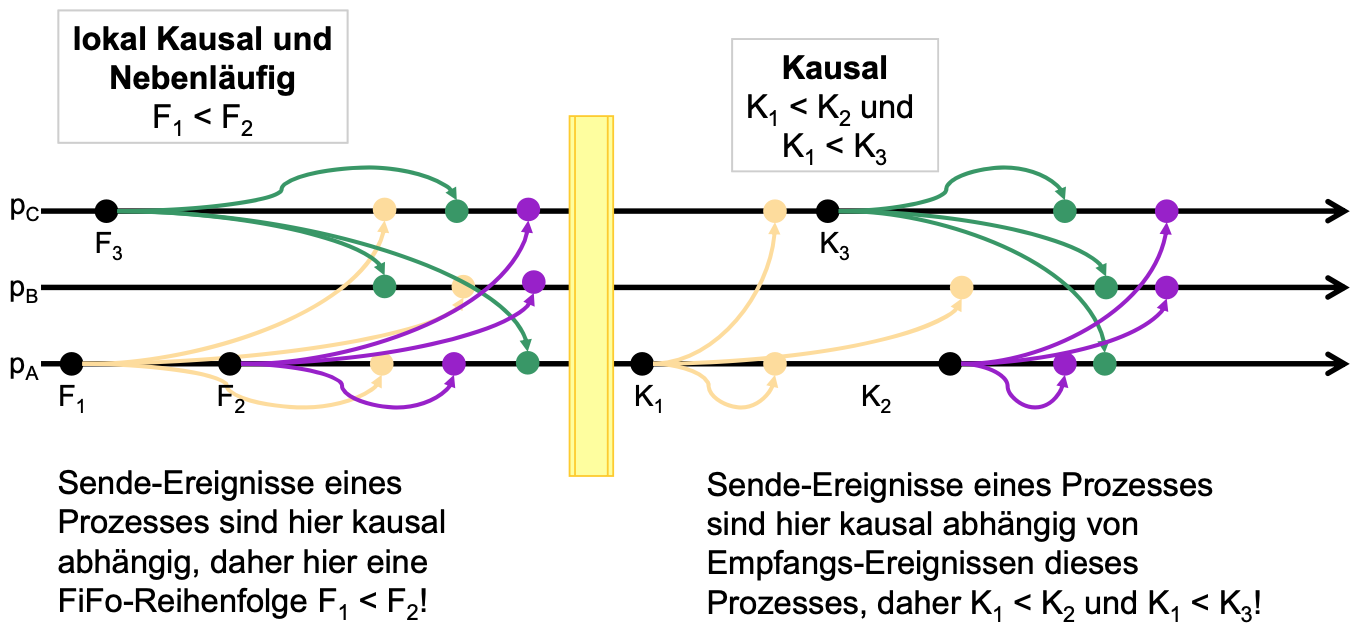
\includegraphics[scale=0.25]{Latex/Bilder/Test1_2.png}
\caption{\label{test1_2} Kausalitätstest 1 und 2 \cite{Aufgabenstellung}}
\end{center}
\end{figure}

Im linken Test \textit{'lokal Kausal und Nebenläufig'} werden die Nachrichten F1 und F2 nebenläufig zueinander von zwei verschiedenen Prozessen aus gesendet. Kausal abhängig ist hier nur die Nachricht F2 von F1. F2 wird erst verschickt, wenn F1 verschickt wurde. In Prozess B ist also wichtig, dass F1 vor F2 ausgeliefert wird. Wann genau F3 ausgeliefert wird ist nicht weiter relevant.

\begin{figure}[htbp]
\begin{center}
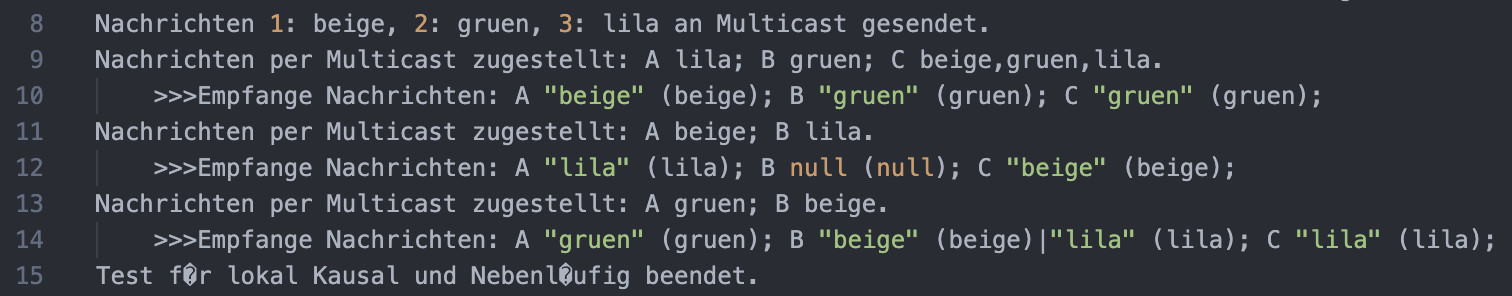
\includegraphics[scale=0.55]{Latex/Bilder/test1_1_results.png}
\caption{\label{test1_2_result} Ergebnisse 3}
\end{center}
\end{figure}

In Abb. \ref{test1_2_result} sind die Logs des Tests zu sehen. Die Nachrichten kommen in folgender Reihenfolge bei den jeweiligen Prozessen an:

\begin{itemize}
	\item \textbf{Prozess A}  $F1 \rightarrow F3 \rightarrow F2$
	\item \textbf{Prozess B} $F3 \rightarrow F1 \rightarrow F2$
	\item \textbf{Prozess C} $F3 \rightarrow F1 \rightarrow F2$
\end{itemize}

$F1 < F2$ ist bei allen Prozessen eingehalten. F3 ist bei Prozess A und bei Prozess B an unterschiedlichen Stellen. Dies zeigt sowohl das Einhalten der kausalen Ordnung, als auch die Nebenläufigkeit.

\subsection{Komplexitätsanalyse}

\subsubsection{Kommunikationseinheit}

Die Komplexität der Kommunikationseinheit hängt im wesentlichen von der Funktion \textit{checkQueues/4} ab. Diese greift auf folgende Funktionen zu:
\begin{itemize}
    \item \textit{vectorC:myVTvc/1} mit einer Komplextität von $O(1)$
    \item \textit{vectorC:aftereqVTJ/2} mit einer Komplexität von $O(m+n)$ (siehe Kapitel \ref{aftereqVTJ_complexity})
    \item \textit{pushDLQ/2} mit einer Komplexität von $O(1)$
    \item \textit{removeFromList/2} mit einer Komplexität von $O(n^2)$
\end{itemize}

Durch die Funktionen \textit{vectorC:aftereqVTJ/2} und \textit{removeFromList/2} ergibt sich $O(n^2)+O(n^2)=O(n^2)$. Die rekursive Tiefe ist $O(n)$, wodurch eine Gesamtkomplexität von $O(n)*0(n^2)=O(n^3)$ für die Funktion \textit{checkQueues/4} resultiert.

\subsubsection{Vektoruhr-ADT}

Die beiden komplexeren Funktionen dieses Moduls sind \textit{compVT/2} und \textit{aftereqVTJ/2}. 

\paragraph{\textit{compVT/2}}

Die genutzte Hilfsfunktion \textit{padWithZeros/2} hat eine Komplexität von $O(m)$. $m$ ist die Länge des resultierenden Vektors.\\
Die zweite genutzte Hilfsfunktion ist \textit{compareLists/2}. Es werden zwei Listen elementweise verglichen, wodurch eine Komplexität von $O(n)$ resultiert. $n$ ist die Länge der Vektoren, welche durch das Padding die gleiche Länge haben.\\
Die Gesamtkomplexität dieser Funktion ist also $O(m+n)$. $m$ und $n$ sind die Längen der beiden übergebenen Vektoren.

\paragraph{aftereqVTJ/2} \label{aftereqVTJ_complexity}

Die erste genutzte Hilfsfunktion ist \textit{removeJ/2}. Diese nutzt die im vorgehenden Paragraphen beschriebene Hilfsfunktion \textit{padWithZeros/2}. Danach wird durch eine Liste iteriert ($O(n)$) und an einen Akkumulator angehängt, was zu $O(k)$ führt. $k$ ist die Länge des Akkumulators. Es folgt eine Komplexität von $O(n)+O(n)+O(n^2)+O(n^2)=O(n^2)$.\\
Die zweite genutzte Funktion ist \textit{compVT/2}. Wie auch im vorherigen Paragraphen beschrieben ist dessen Komplexität $O(m+n)$, bzw. $O(n)$, da die beiden übergebenen Vektoren die gleiche Länge haben.\\
Es ergibt sich eine Gesamtkomplexität von $O(n^2)+O(n)=O(n^2).$

\subsubsection{Ungeordneter Multicast}

Die maximale Gesamtkomplexität aller Schnittstellen in diesem Modul ist $O(n)$.

\subsubsection{Vektoruhr Zentrale/Tower}

Die maximale Gesamtkomplexität aller Schnittstellen in diesem Modul ist $O(n)$.